\documentclass[]{standalone}
\usepackage{../NHQMReport/main/NHQM}

\newcommand\proton[1]{%
\shade[ball color=red] (#1) circle(0.5);
}

\newcommand\neutron[1]{%
\shade[ball color=blue] (#1) circle(0.5);
}
\begin{document}
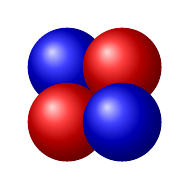
\begin{tikzpicture}

\neutron{-0.35,0.35}
\proton{0.35,0.35}
\proton{-0.35,-0.35}
\neutron{0.35,-0.35}
	

\end{tikzpicture}
\end{document}

	%   \centering
	%     \tikzstyle{ne}=[circle, draw, minimum size=1.25cm, fill = blue]
	% \tikzstyle{pr}=[circle, draw, minimum size=1.25cm, fill = red]
	% 
	%       \begin{scope}[]
	%         \node[pr] ( ) at (-0.35, 0.35  ) {};
	%         \node[ne] ( ) at (0.35,  0.35 ) {};
	%         \node[ne] ( ) at (-0.35,  -0.35 ) {};
	% 
	%         \node[pr] ( ) at (0.35,  -0.35 ) {};
	% 	]	
	% 	
	% 	
	%       \end{scope}
	%     \end{tikzpicture}